\normalsize
\begin{FlushLeft}
    \section{Technical Design}

    \subsection{Programming Language Selection and Libraries Used}

    I selected C# as my programming language for several reasons. Currently, it is the language that I am most familiar with. In addition, I conducted research on which languages are best for fast processing, and found that C, C++, and C# are among the top contenders. Considering my skill set and the importance of speed in this situation, I concluded that C# would be a good fit. Furthermore the object orientated nature of the language means that I will be able to separate the front end and the back end processing into separate bll files keeping the code clean and easily maintainable.\\ 
    \bk
    Find below a list of all libraries I used: \\
    
    \subsubsection{Linq}
    In order to manipulate lists and create the data structures that I need I will need to use some Linq methods. During the prototyping stage I found that using some Linq methods such as the Select statement allowed the program to be easier to read and make logical sense. As well as this there have been optimisations made in the iterative Linq methods which will make my program faster. Similar to some of the following libraries this is a Microsoft Library which is open source.
    \\ \bk


    \subsubsection{Bitmap}
    In order for my program to function a required part of it is that it is able to take an image as an input. In native C# there is no set way to do this. Therefore I needed to use the Microsoft System.Drawing Namespace. This namespace provides access to GDI+ basic graphics functionality. This does limit this project as is to only working on Windows since the library requires access to the GDI+ native library which is only on windows services. \\
    
    The only part of this library I will be using is the Bitmap class. This will allow me to accept all types of images without the need of parsing them myself since this is not the aim of my project. 
    \\ \bk

    \subsubsection{Windows Forms}
    In order to complete my objectives my program will need to be easy to use and any user with some degree of technical competency should be able to use it. In order to achieve this objective I though that instead of using some form of console input in order to get a starting and an end location, that it would be better to use some form of GUI. In order to do this I will use Windows Forms. This will allow me to make a simple GUI which will allow the end user to interact with the user and easily understand. \\ 

    The things which I will end up using the windows forms are the map traversal, allowing the user to select a start and an end node with a click instead of having to enter a coordinate. As well as this I will also use forms to show the user the stages of, for example, the canny edge detection.
    \\ \bk

    \subsection{High Level Overview}
    The general purpose of my project is to allow a user to take a map and input it into my program, then subsequently convert it into a routable map. \\ \bk
    
    In order to achieve this goal my program will first take an input, the users map. It will then take this map and convert it into an machine readable format, a Bitmap. Canny edge detection will then be performed on it causing the edges and the surroundings of the paths on the image to be found. Using these edges a filling algorithm will fill the spaces encapsulated by the lines. Finally these filled spaces will be used to convert the whole image to a graph which can then be traversed using graph traversal algorithms such as A* or Dijkstra's algorithm. \\ \bk

    \begin{figure}[H]
        \centering
        \subfloat[\centering High Level Overview Of Program]{{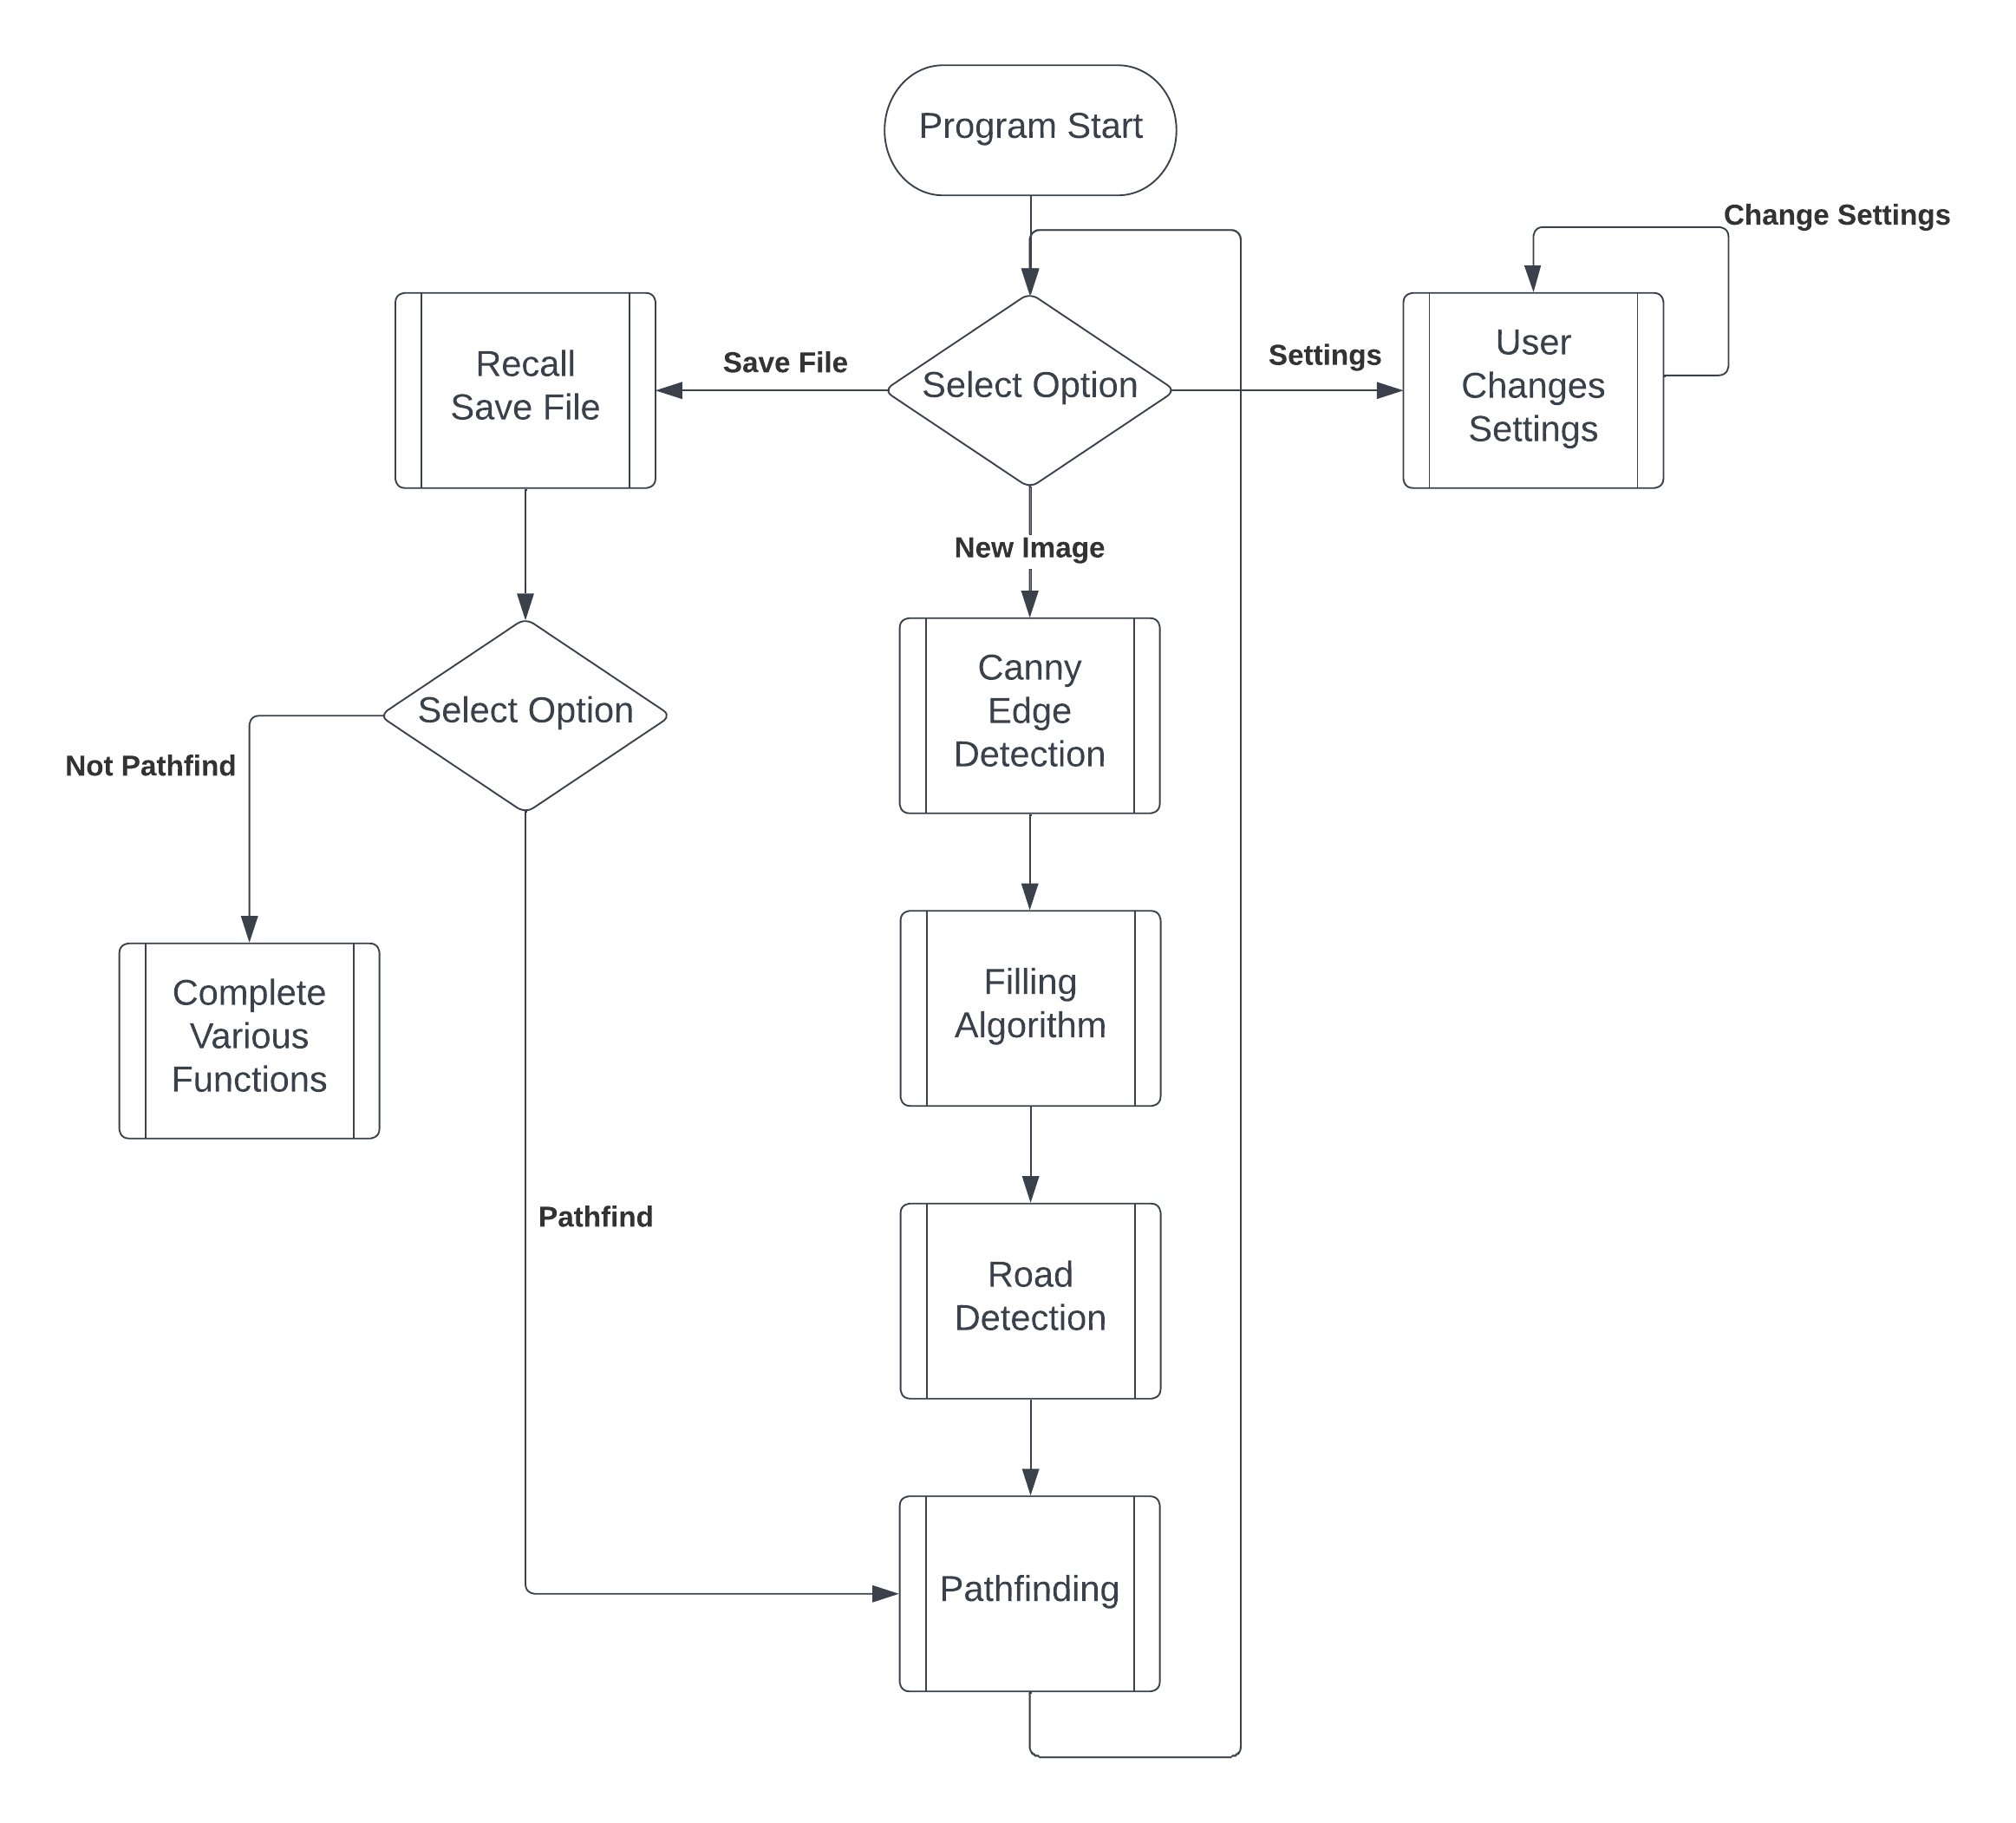
\includegraphics[width=17.2cm]{images/HighLevelOverview.png}}}
    \end{figure}

    The version of Edge Detection I will be using as previously stated will be Canny Edge Detection, this is as opposed to Sobel Edge Detection. The main version of filling I will be using is flood fill due to it simple nature to implement ad due to the fact that it does not take much memory and can be made recursive so it performs well. The final main algorithm I will need to use is image kernels and convolution, this will allow me to manipulate the inputted image.

    \subsubsection{Backend Library}
    For my project to ensure that I conform to the OOP principle of encapsulate what varies. I will accomplish this through the use of classes and encapsulation. Furthermore I have also made the decision to split up my solution into two separate projects, this means that my program will produce two files in order to run, one of these will be the DLL for the backend library and the other will be the executable for the front end. \\ \bk

    Contained within this backend section of my program will be contained the edge detection, road detection, complex data types and graph traversal algorithms as well as various utilities that are frequently used throughout the program. \\ \bk

    One of the main features of the backend library are the custom structures that have been created in order to allow for easier processing of data. Find below the image of the structure class layout and the classes which link within.

    \begin{figure}[H]
        \centering
        \subfloat[\centering Overview of Backend Structures]{{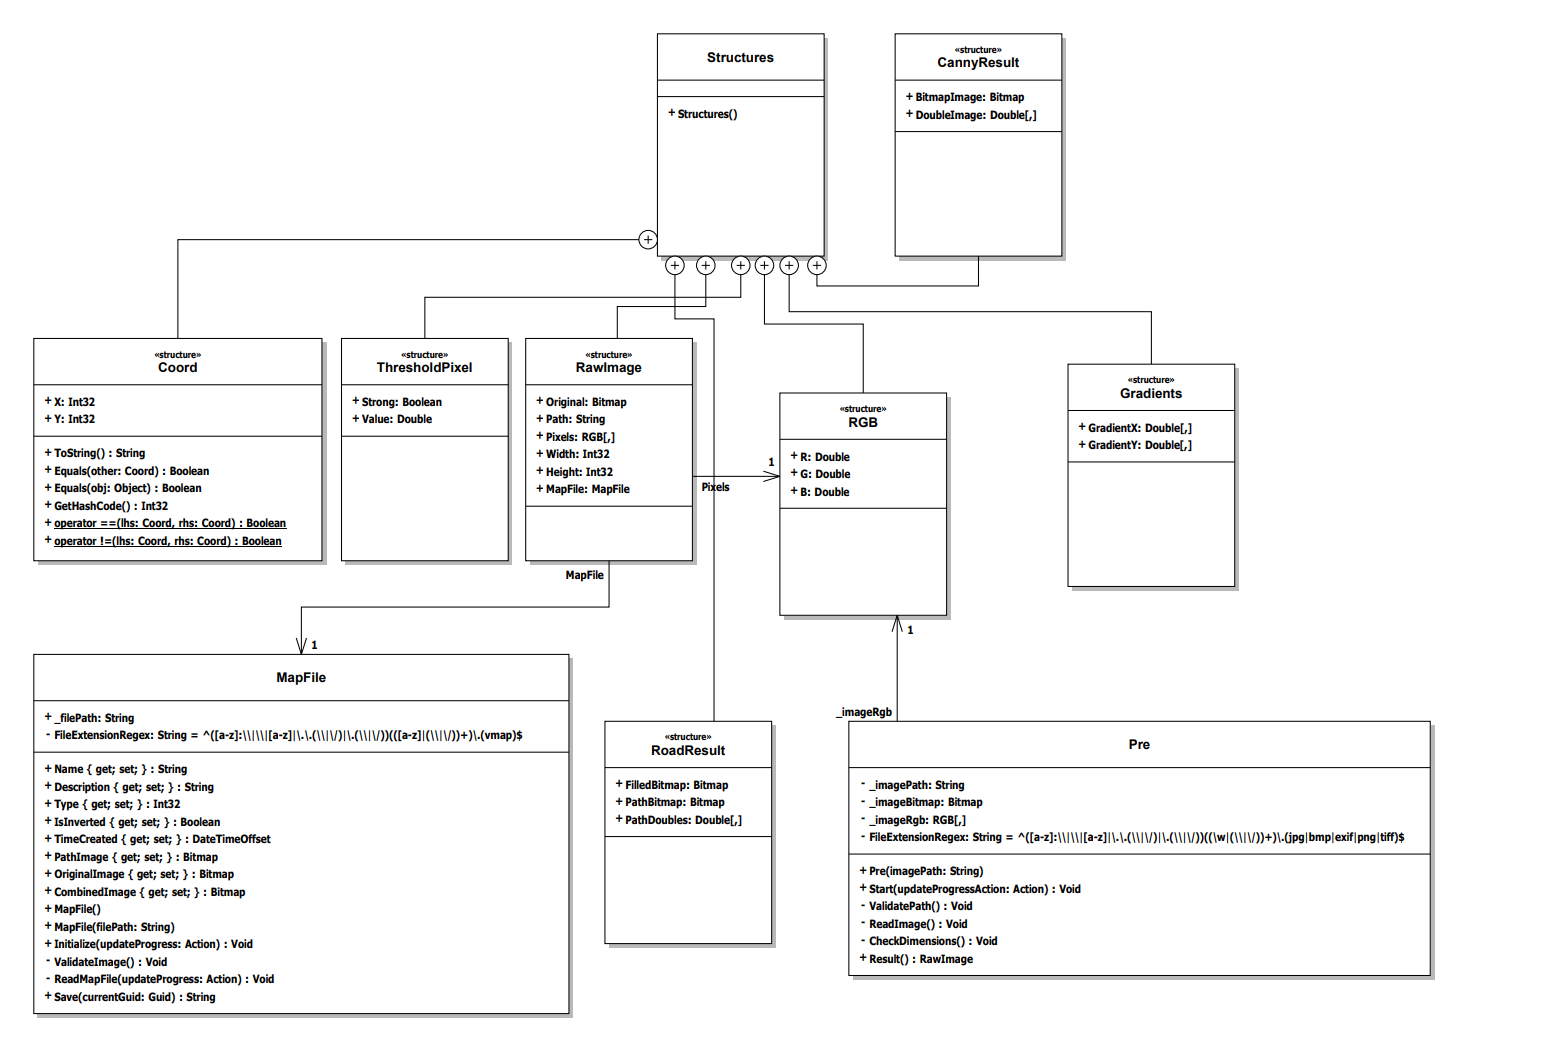
\includegraphics[width=17.2cm]{images/UML/Backend.png}}}
    \end{figure}

    \\

    As can be seen form the class diagram of the backend library, there is very little dependency within the library itself. This allows the backend to function independently of the program which is using it. This allows the backend to be split out and moved to another program if needed. Summarised there are four main reasons to do this:

    \begin{enumerate}
        \item \textbf{Modularity} - By separating the backend from the frontend one is able to be built without the other. This means that when working on my project I can take time to perfect one without impacting the other.
        \item \textbf{Reusability} - As previously stated being able to be reused is a large reason as to why to separating the elements is a good idea. Since if I wanted to expand this project for example and make a web interface for it, I could take the maths of the backend and recreate the front end in a web framework like Razor Pages.
        \item \textbf{Maintainability} - It is allot easier to maintain code when it has been organised into classes and by extension into libraries where a library is a collection of classes. It means that should something throw an error in the backend I would be able to easily isolate the issue and be able to fix it.
        \item \textbf{Testability} - In a similar vain to the Maintainability of the program being modular also means that it is very easy to implement testing. This means that as I go thorough making my program it will make it allot easier to separate variables and make isolated testing conditions. Furthermore it means that I can test the maths of the Canny Detection without having to worry about making an interface to it using the UI.
    \\ \BK

    \subsubsection{Local Application}
    The local application part of this program will be responsible for the tying if the various algorithms of the backend together along with providing the user with a way to interact with them, whether this is through the use of windows forms of the console for text inputs. As stated by objective 5 the design of the UI should be simplistic and easy to understand at a glance, therefore I will only be using the methods as stated above for interacting with the user. I also believe that it will be best to keep the changes between the two to a minimum and when there is a change make sure that the user is aware of it before hand.\\ \bk
    
    \paragraph{Design of User Interface (Console)} \mbox{} \\
    In order to keep the user interface as easy to use as possible the console will remain static while the program is being run. This means that once it has been started and set to its correct size it will form itself to fit the screen and will only run if it has been maximized. This will allow me to make sure that the interface is clear and easy to use. Find below a mock-up of the console design.
    
    \begin{figure}[H]
        \centering
        \subfloat[\centering Mock-up of Console Interface]{{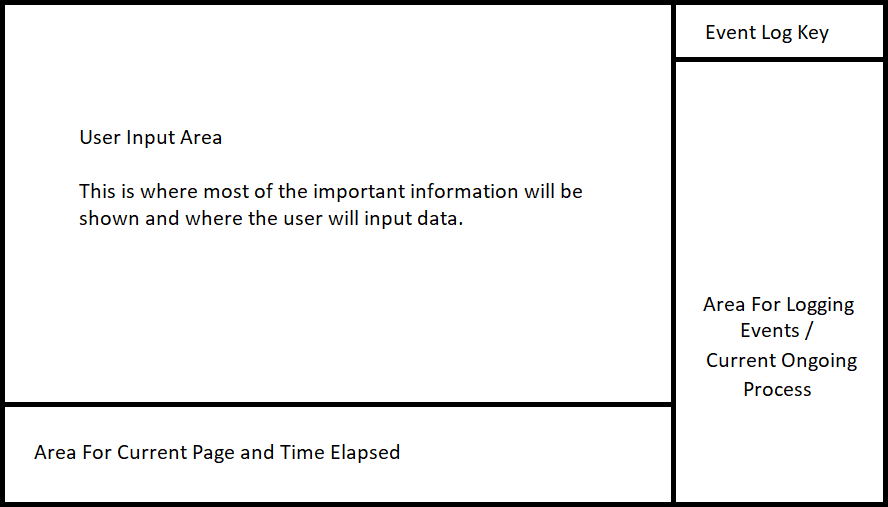
\includegraphics[width=12.5cm]{images/design/consoleMock.png}}}
    \end{figure}\\

    As can be seen in this mock-up fo the console interface it can be seen that there is a large section for the user to enter and view important in. As will be expanded on in the second section about the Windows Forms interface, due to the static nature of the console I will be able to make a Form conform to the shape of this area. See the next paragraph for more information. \\ \bk

    As for the other elements of the console UI, as part of objective 5, this must be easy to see at a glance what is going on and which step you are in. To accomplish this on the right hand side of the console there will be a log which, should the user select to do so in settings, will display each method call and the result of that call allowing them to see exactly where they are in the process. \\ \bk
    
    At the bottom of the console in the section labelled "Area for Current Page and Time Elapsed" this will be used for, as the name suggests, the current page and time elapsed. What this means is that at a glance a non-technical user or one who has opted not to have the advanced logging will still be able to see where they area at in the current process. \\ \bk

    \begin{figure}[H]
        \centering
        \subfloat[\centering Mock-up of Console Interface]{{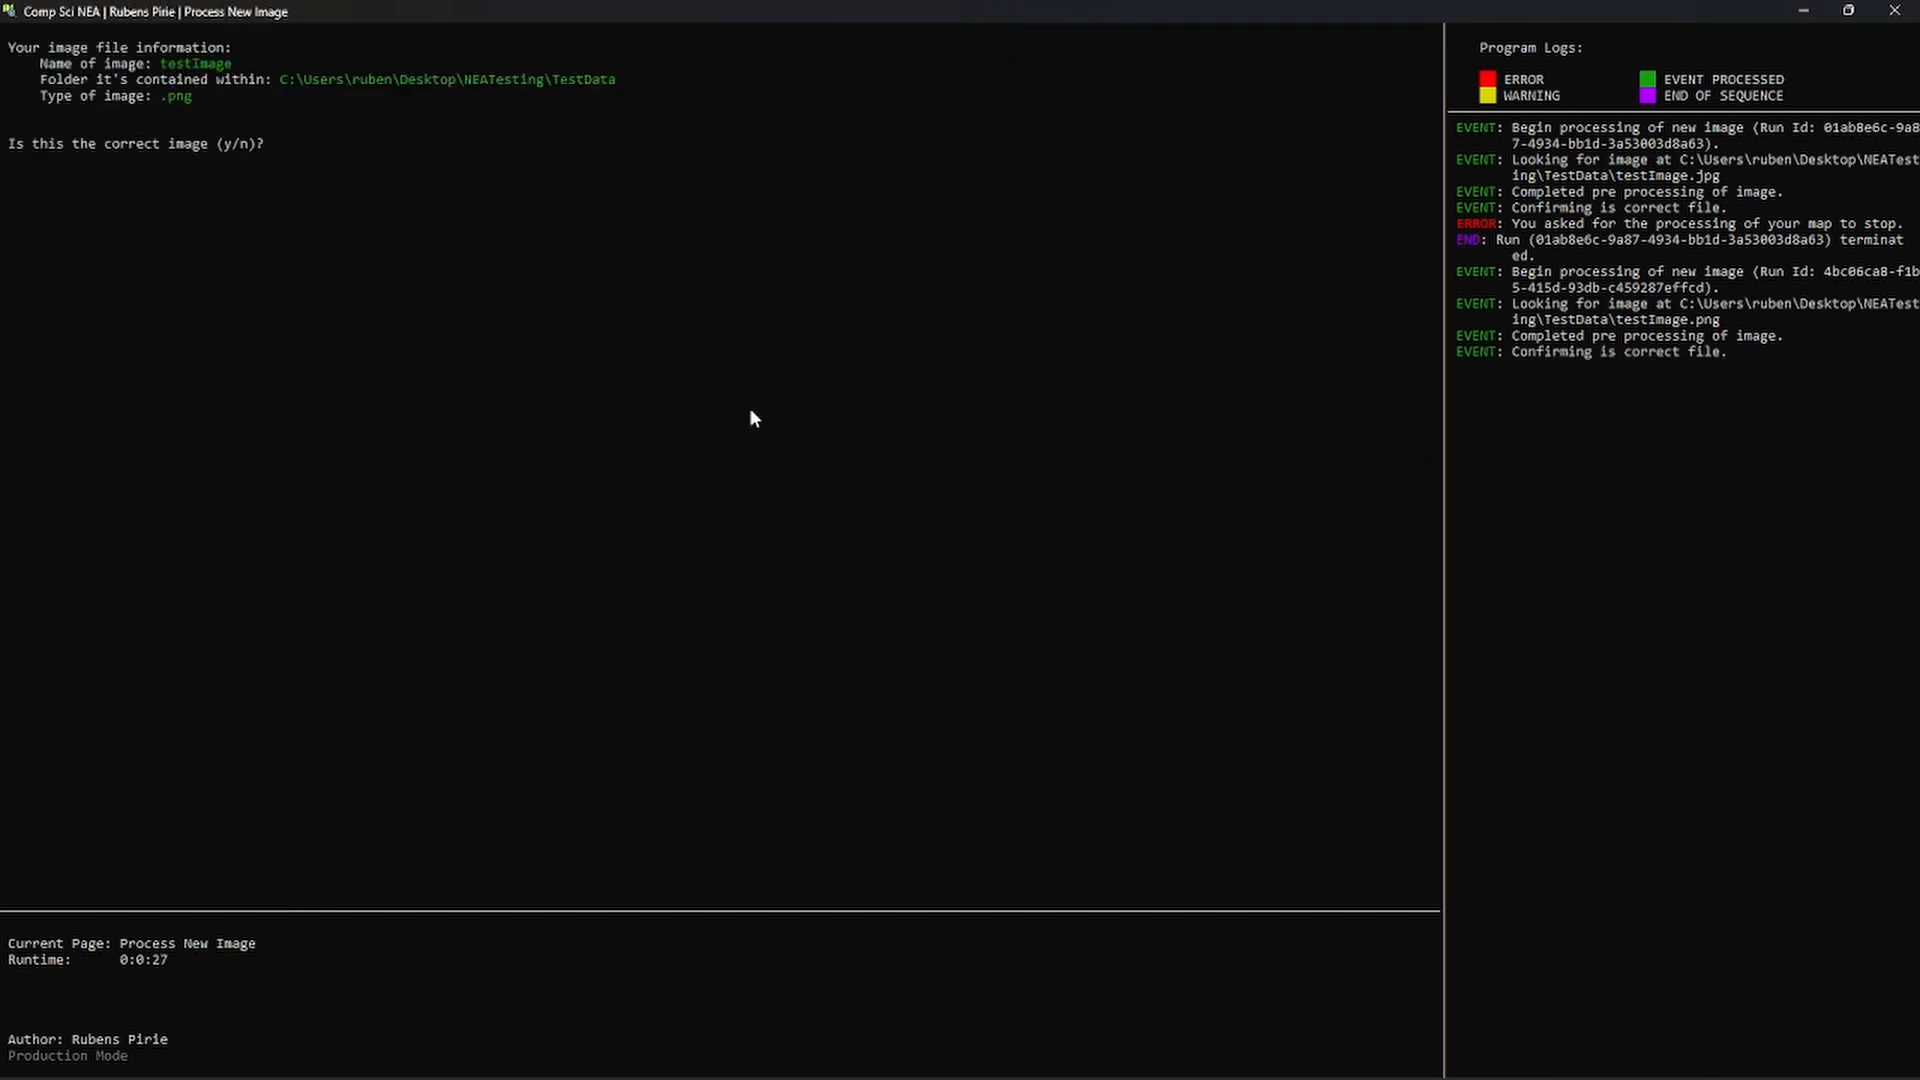
\includegraphics[width=12.5cm]{images/design/terminal.png}}}
    \end{figure}\\
    
    \BK

    \paragraph{Design of User Interface (Windows Forms)} \mbox{} \\
    For the forms interface I have chosen to keep the use of the opening of new windows to a minimum, as explained above I want this part of the program to be as simple as possible to avoid over stimulating the user and confusing them. 

    \begin{figure}[H]
        \centering
        \subfloat[\centering Windows Form For Confirming Image]{{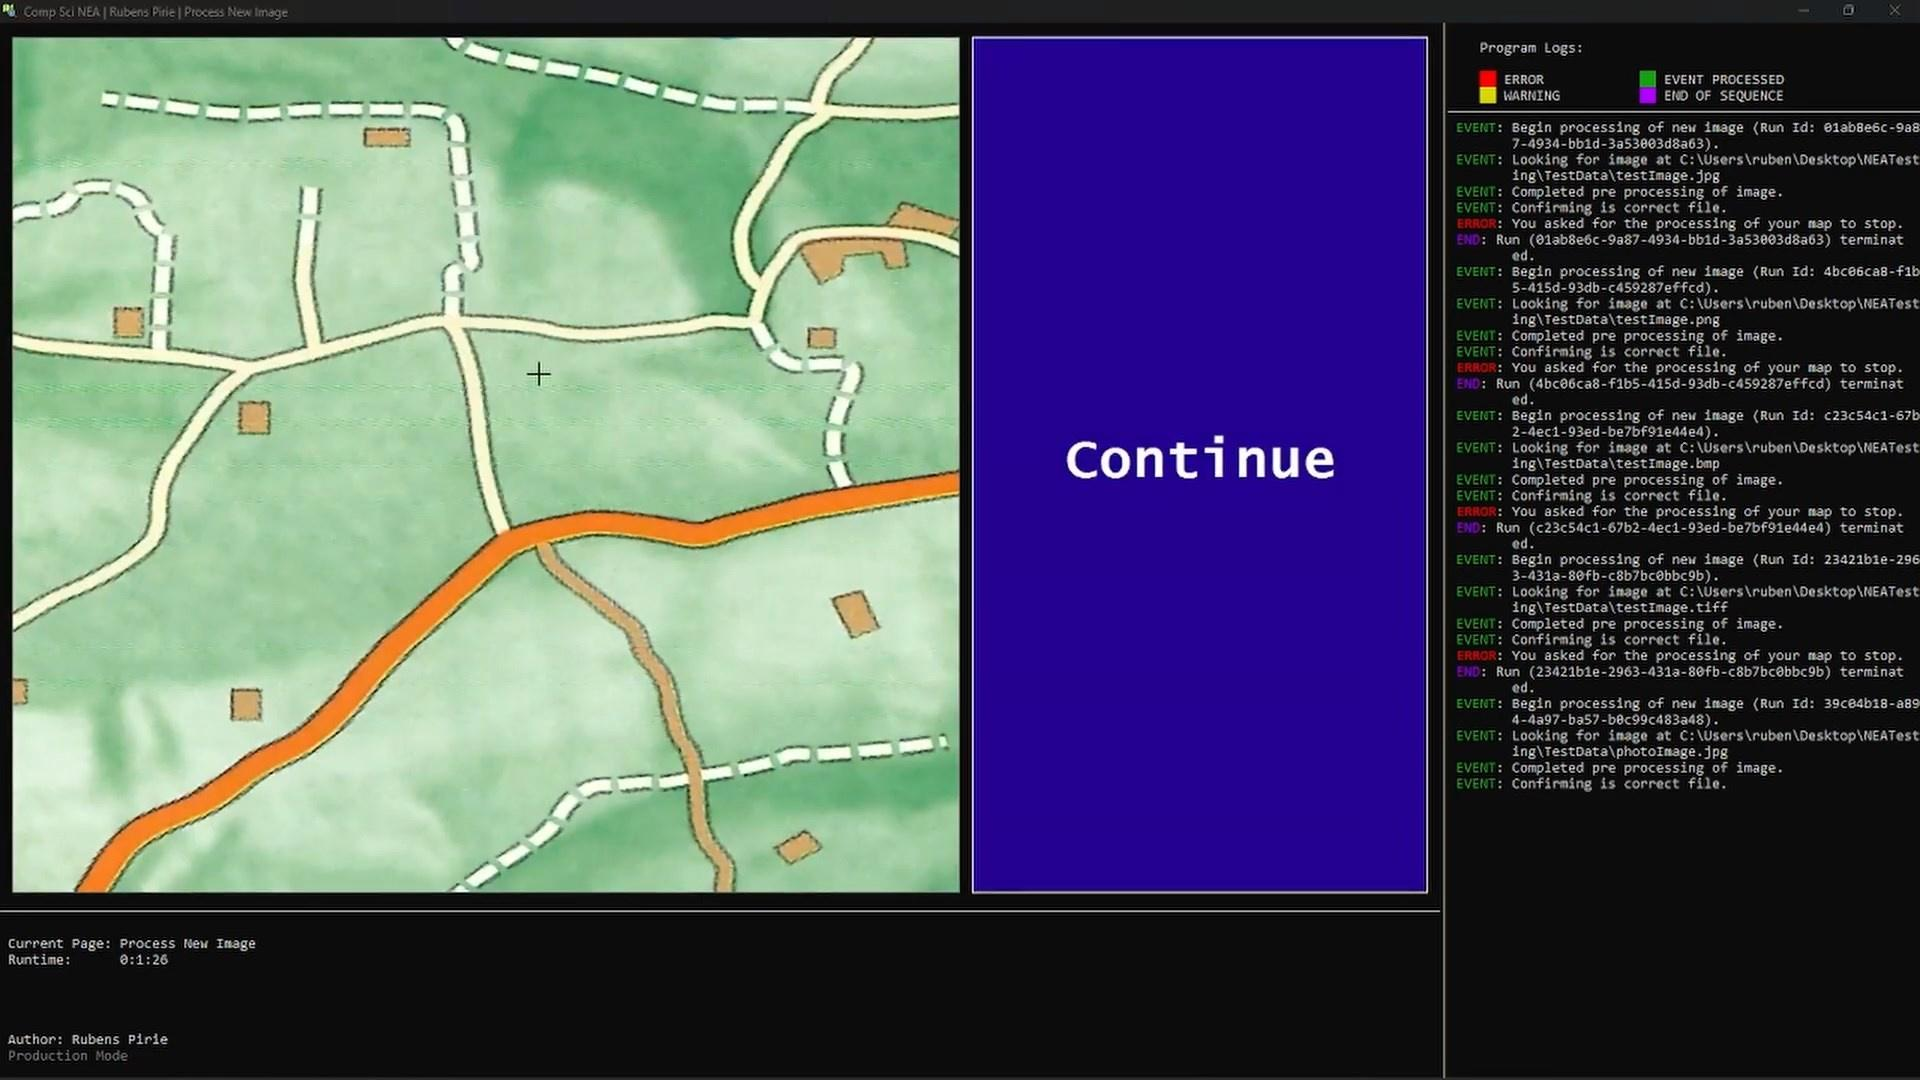
\includegraphics[width=12.5cm]{images/design/confirmWindow.jpeg}}}
    \end{figure}\\

    \begin{figure}[H]
        \centering
        \subfloat[\centering Windows Form For Pathfinding Image]{{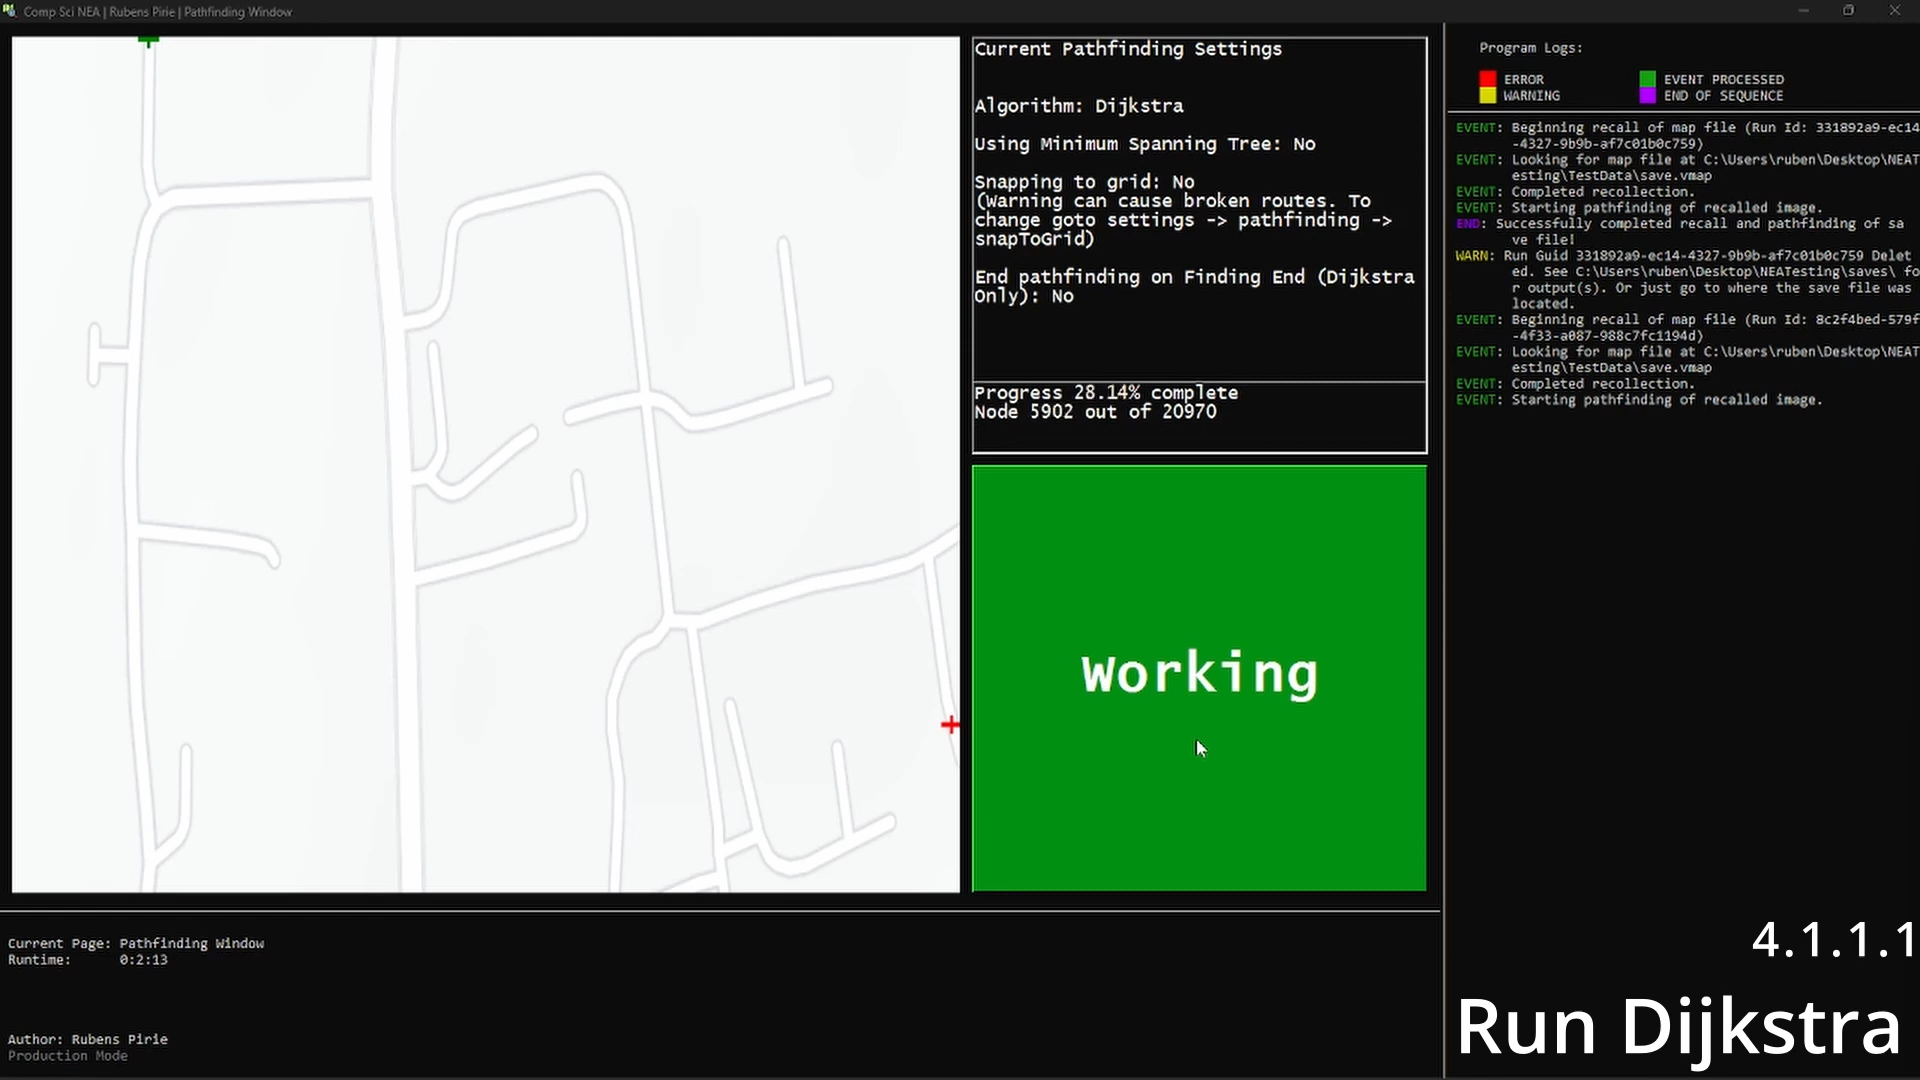
\includegraphics[width=12.5cm]{images/design/pathfindWindow.png}}}
    \end{figure}\\

    \\ \BK


    \\ \bk

    \subsection{Class Overviews}

    In this following part of the write up will go briefly over every class in the program first stating its function, which section it is in (backend library or front end application) and finally how it plays a part in the program.

    \paragraph{Async Edge Detection \textit{(Class)}} \mbox{} \\

    \begin{figure}[H]
        \centering
        \subfloat[\centering Async Edge Detection Class Diagram]{{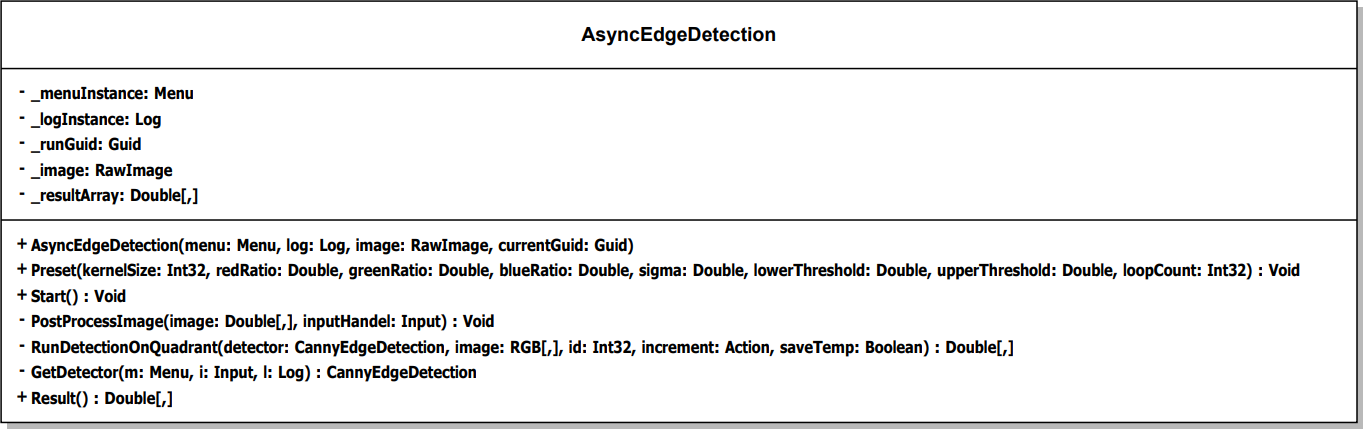
\includegraphics[width=16cm]{images/UML/AsyncEdgeDetection.png}}}
    \end{figure}\\

    This class is located in the front end section of my application, its main function is to coordinate the method calls of the Canny Edge Detection class. Due to the separated nature of my program I did not want there to be any user inputs in the accrual processing section. In order to do this I needed to have a separate hander on the local application side which would ask the user for their inputs and handel all of the validation of them. \\ \bk

    This class also implements the IHandler interface, this is to allow the main front end application to switch between the Async version and the Synchronous version of the edge detection without having a mess of IF statements. Part of the IHandler interface means that this class must contain the methods, Start() and Result(). What these methods do is what they say in the name. The start methods begins the process of getting user inputs and then starting the edge detection. The Result method will, as the name suggests return the result of the edge detection. \\ \bk

    The PostProcessImage method in the class is responsible for the custom embossing which runs through the result of the canny edge detection and fills in any gaps that may have appeared. It also applies an embossing kernel on the image to embolden the lines. It will also prompt the user to enter the amount of times they want to run the embossing process. \\ \bk
    
    The GetDetectorMethod is used to get the variables for the canny edge detector. This section handles all of the validation and checking that the values supplied are valid. The result of this method is that a new Canny Edge Detector object is created with the user inputted variables, this is then passed down the chain to be used in processing each quadrant. \\ \bk

    The main differentiator between this asynchronously method and the synchronous method is that this one will split the input image into 4 distinct quadrants, this will allow the program to run each at the same time using threading. Through my prototyping stage I found that using this method of threading greatly improves the speed even on lower specification computers. \\ \bk
    
    Finally the Preset method is used in the front end application in the eventuality of the user selecting preset values. An example of this is that when it gets to the selection of the edge detection method they select the "Photograph" method, the async method will be used due to its speed however instead of prompting the user it will run the various stages with predefined values. \\

    \bk


    \paragraph{Canny Edge Detection \textit{(Class)}} \mbox{} \\

    \begin{figure}[H]
        \centering
        \subfloat[\centering Canny Edge Detection Class Diagram]{{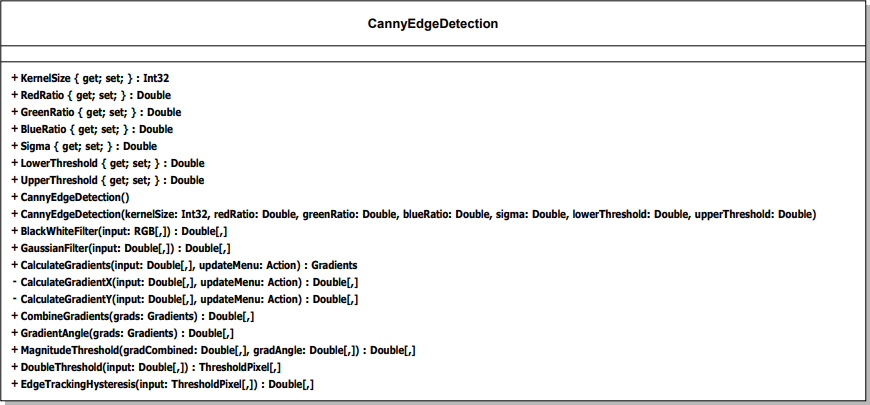
\includegraphics[width=16cm]{images/UML/CannyEdgeDetection.png}}}
    \end{figure}\\

    This class is located in the backend library portion of my project, its main function is to house the methods which contain the maths to perform the canny edge detection. Since this method is in the backend library of my project there is no user input here however in many of the methods an action is passed in, this is used to update the progress bar on the front end without having the two intrinsically integrated. \\ \bk

    The first set of methods shown in the class diagram are in essence properties on the class which are used in the various calculations. The reason that I will go with getter and setter variables is that if at some point in the future I wish to restrict access to the properties on the class or perhaps mutate the way in which they are stored this could be easily done without the need to change many different things. \\ \bk

    The first method and subsequently the first stage in canny edge detection is the black and white filter. The default behaviour is that it uses the industry standard for getting a single value from a RGB pixel which is as follows $$ Y' = 0.299R' + 0.587G' + 0.114B' $$.  It will perform the same calculation for every pixel in the supplied image causing it to be converted to black and white. This is used since if the detection was run on each colour chanel seperatly this would not give one unified result and could be very inaccurate.\\ 

    \\ \bk

    The next method in this class is the Gaussian Filter this will pass over the image and apply a Gaussian Filter kernel to each pixel. This is mainly used in order to make sure that any noise in the image is suppressed to avoid false edges. The maths for the kernel implementation and matrix convolutions are covered in their respective classes as well as the gaussian equation. A rough approximation for the gaussian kernel is as follows:\\

    \begin{gather*}
        \frac{1}{159}\begin{pmatrix}
            2 & 4 & 5 & 4 & 2 \\
            4 & 9 & 12 & 9 & 4 \\
            5 & 12 & 15 & 12 & 5 \\
            4 & 9 & 12 & 9 & 4 \\
            2 & 4 & 5 & 4 & 2
        \end{pmatrix}
    \end{gather*} \\

    It is stated that the larger the kernel is the less effect noise will have on the result however it will impact the performance of the detector, for this reason the Canny Edge Detection class defaults to a kernel size of 5x5. \\ \bk

    The next stage of canny edge detection involve calculating gradients and gradient angles and for this reason I will be combining the CalculateGradients, CalculateGradientX and CalculateGradientY into one. Again another way in which I will optimise the canny edge detection is by using threading. In order to calculate the gradient direction I will need to use Atan2, this requires an X and Y component which are independent of each other, a perfect use of threading. When a image gets to this point it will be processed at the same time by each method. The process completed by each method is vastly the same they will just be applying different image kernels, both are the sobel edge kernels keeping with the scheme of canny edge detection. \\ \bk   

    \begin{center}
        
        $
        M_x = \begin{pmatrix}
            +1 & +2 & +1 \\
            0 & 0 & 0 \\
            -1 & -2 & -1
        \end{pmatrix}
    $ 
    and $ M_y = \begin{pmatrix}
            +1 & 0 & -1 \\
            +2 & 0 & -2 \\
            +1 & 0 & -1 
        \end{pmatrix}
    $
    \end{center} \\
 
    \bk

    Once the gradient magnitudes in each dimension have been calculated the result of these can be fed into the CombineGradients method. This method will finally extract the usefully data which has been created from applying the two sobel gradient kernels. The first of these is working out the combined gradient magnitudes which is simply calculated with the equation: \\
    
    \begin{gather*}
        G = \sqrt{G_x^2 + G_y^2}
    \end{gather*} \\
    
    We then also want to calculate the direction in which the gradient is travelling to work out if it is extreme enough to quantify an edge. This is achieved though the use of Atan2 as follows:\\
    
    \begin{gather*}
        \Theta = \text{Atan2}(G_x, G_y)
    \end{gather*} \\ 

    \bk

    The next stage in canny edge detection is gradient magnitude threshold's, this is a method of removing lines which would not be "thick enough" to be a propped edge. This is accomplished by the use of the MagnitudeThreshold method and the bullet point description: \\ 
    
    At every pixel N in a given image, it will be suppressed (removed) if,
    \begin{itemize}
        \item the rounded gradient angle is 0° (i.e. the edge is in the north-south direction) the point will be considered to be on the edge if its gradient magnitude is greater than the magnitudes at pixels in the east and west directions.
        \item the rounded gradient angle is 90° (i.e. the edge is in the east-west direction) the point will be considered to be on the edge if its gradient magnitude is greater than the magnitudes at pixels in the north and south directions.
        \item the rounded gradient angle is 135° (i.e. the edge is in the northeast-southwest direction) the point will be considered to be on the edge if its gradient magnitude is greater than the magnitudes at pixels in the north-west and south-east directions.
        \item the rounded gradient angle is 45° (i.e. the edge is in the northwest-southeast direction) the point will be considered to be on the edge if its gradient magnitude is greater than the magnitudes at pixels in the north-east and south-west directions.

    \end{itemize}
    
    \\ \bk

    The penultimate method call is to Double Threshold suppression. After the magnitude threshold, remaining edge pixels provide a more accurate representation of real edges in an image. However, some edge pixels remain that are caused by noise and color variation which didn't get removed by the gaussian filter stage. To account for these spurious responses, it is essential to filter out edge pixels with a weak gradient value and preserve edge pixels with a high gradient value. \\

    The way in which this is implemented is that a user threshold from the beginning is used and if the pixel is greater than the threshold then it is included, if it is below the max threshold but greater than the min then it is set to a strong pixel and retains its value. In any other case it is removed and its value is set to 0. \\ \bk

    Finally edge tracking by hysteresis is used, to track the edge connection, blob analysis is applied by looking at a weak edge pixel and its 8-connected neighbourhood pixels. As long as there is one strong edge pixel that is involved in the blob, that weak edge point can be identified as one that should be preserved. These weak edge pixels become strong edges that can then cause their neighbouring weak edge pixels to be preserved otherwise they are not preserved and are removed. After each of these sages canny edge detection is complete. \\ \bk    
    \bk


    \paragraph{Canny Result \textit{(Structure)}} \mbox{} \\

    \begin{figure}[H]
        \centering
        \subfloat[\centering Canny Result Class Diagram]{{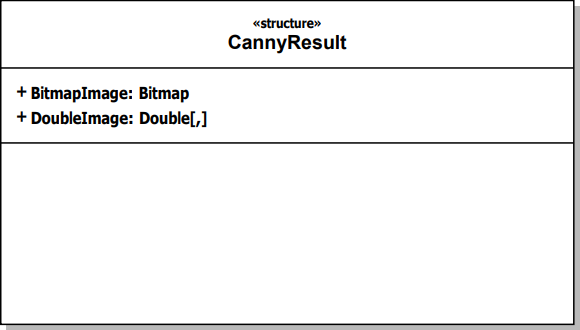
\includegraphics[width=8cm]{images/UML/CannyResult.png}}}
    \end{figure}\\

    This is contained within the static class of structures in the backend library. There is no methods or functions contained within this class since it is in fact a structure. Its main function is to contain any relevant data from Canny Edge Detection.

    \bk

    \paragraph{Coord \textit{(Structure)}} \mbox{} \\

    \begin{figure}[H]
        \centering
        \subfloat[\centering Coord Class Diagram]{{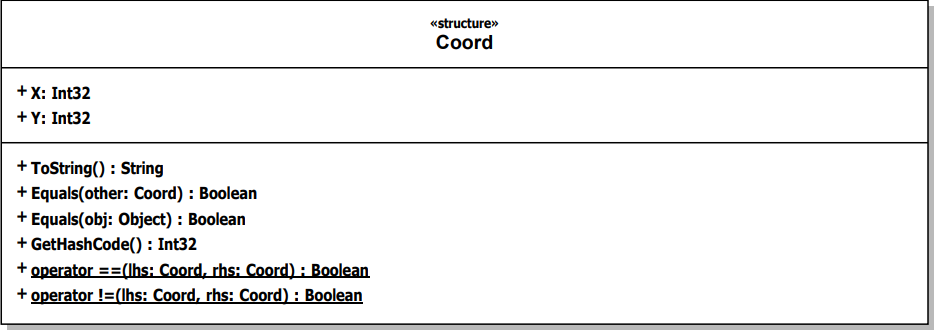
\includegraphics[width=13cm]{images/UML/Coord.png}}}
    \end{figure}\\

    Similar to above this is contained within the static class of structures. It is used to represent a coordinate, and unlike the canny result structure, it does contain methods. The main of which are the operator overloads. This allows me to directly compare two different coordinates instead of constantly comparing each dimensions. The other hash codes and alike are used when a dictionary is required in order for them to be converted into a hash code. Finally the ToString method is mainly used during testing however it can also be used to inform the user of a coordinate that they are interacting with.

    \bk

    \paragraph{Extensions \textit{(Class)}} \mbox{} \\

    \begin{figure}[H]
        \centering
        \subfloat[\centering Extensions Class Diagram]{{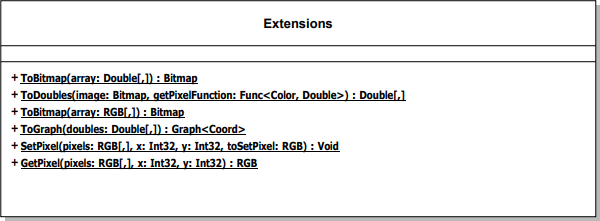
\includegraphics[width=13cm]{images/UML/Extensions.png}}}
    \end{figure}\\

    This class is responsible for altering the default behavior of

    \bk

    \paragraph{Gradients \textit{(Structure)}} \mbox{} \\

    \begin{figure}[H]
        \centering
        \subfloat[\centering Gradients Class Diagram]{{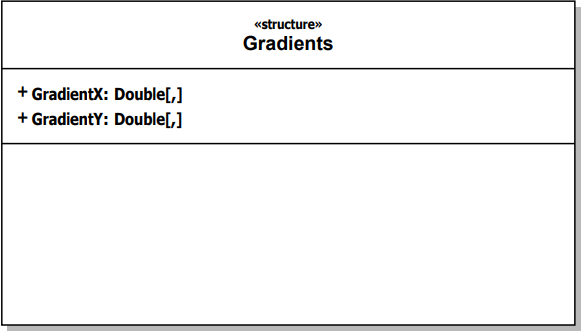
\includegraphics[width=8cm]{images/UML/Gradients.png}}}
    \end{figure}\\

    \bk


    \paragraph{Graph \textit{(Class)}} \mbox{} \\

    \begin{figure}[H]
        \centering
        \subfloat[\centering Graph Class Diagram]{{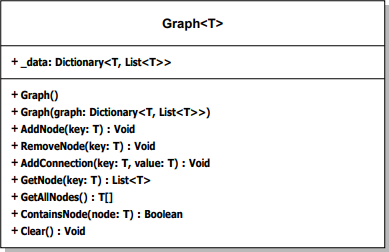
\includegraphics[width=8cm]{images/UML/Graph.png}}}
    \end{figure}\\

    \bk

    \paragraph{Graph Exception \textit{(Exception)}} \mbox{} \\

    \begin{figure}[H]
        \centering
        \subfloat[\centering Graph Exception Class Diagram]{{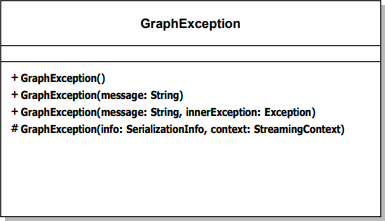
\includegraphics[width=12.5cm]{images/UML/GraphException.png}}}
    \end{figure}\\

    \bk

    \paragraph{IHandler \textit{(Interface)}} \mbox{} \\

    \begin{figure}[H]
        \centering
        \subfloat[\centering IHandler UML Diagram]{{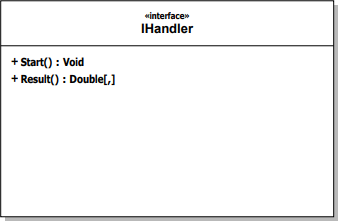
\includegraphics[width=12.5cm]{images/UML/IHandler.png  }}}
    \end{figure}\\

    \bk

    
    \paragraph{Input \textit{(Class)}} \mbox{} \\

    \begin{figure}[H]
        \centering
        \subfloat[\centering Input Class Diagram]{{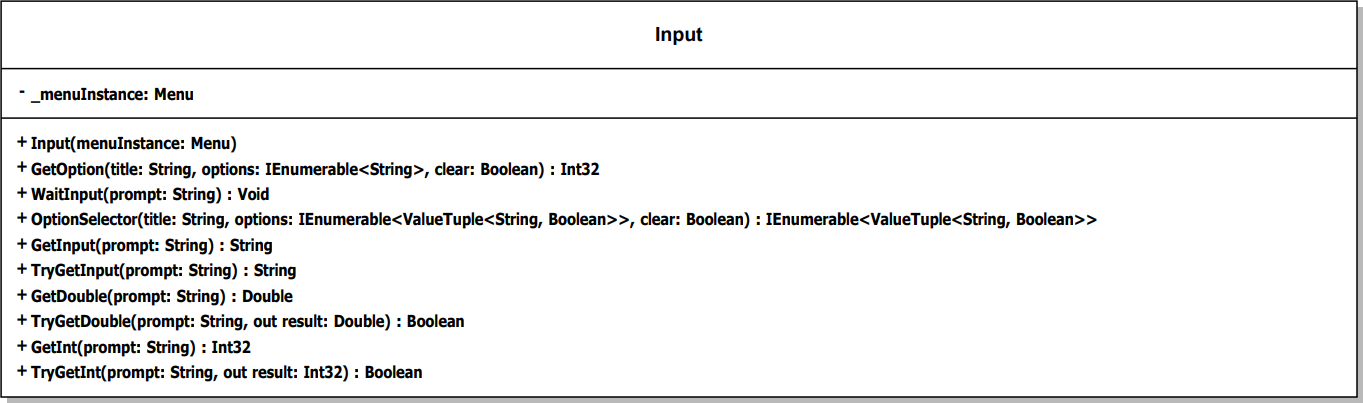
\includegraphics[width=12.5cm]{images/UML/Input.png}}}
    \end{figure}\\

    \bk

    
    \paragraph{Kernel \textit{(Class)}} \mbox{} \\

    \begin{figure}[H]
        \centering
        \subfloat[\centering Kernel Class Diagram]{{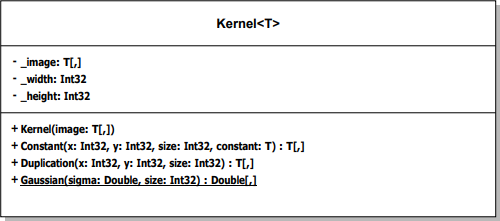
\includegraphics[width=12.5cm]{images/UML/Kernel.png}}}
    \end{figure}\\

    \bk

    
    \paragraph{Kernel Exception \textit{(Exception)}} \mbox{} \\

    \begin{figure}[H]
        \centering
        \subfloat[\centering Kernel Exception Class Diagram]{{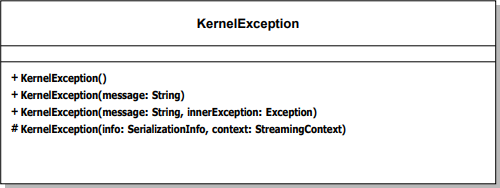
\includegraphics[width=12.5cm]{images/UML/KernelException.png}}}
    \end{figure}\\

    \bk

    \paragraph{Log \textit{(Class)}} \mbox{} \\

    \begin{figure}[H]
        \centering
        \subfloat[\centering Log Class Diagram]{{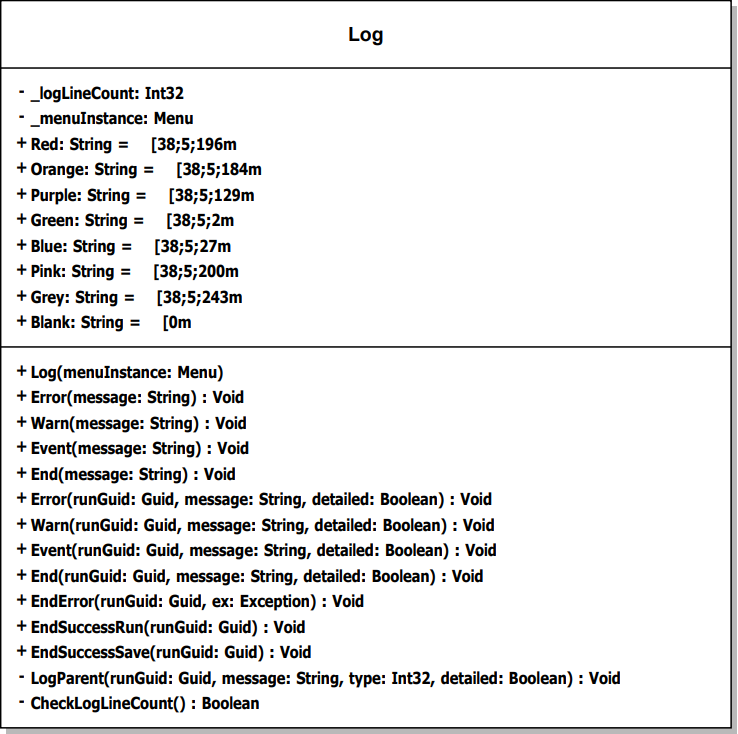
\includegraphics[width=12.5cm]{images/UML/Log.png}}}
    \end{figure}\\

    \bk

    \paragraph{Logger \textit{(Class)}} \mbox{} \\

    \begin{figure}[H]
        \centering
        \subfloat[\centering Logger Class Diagram]{{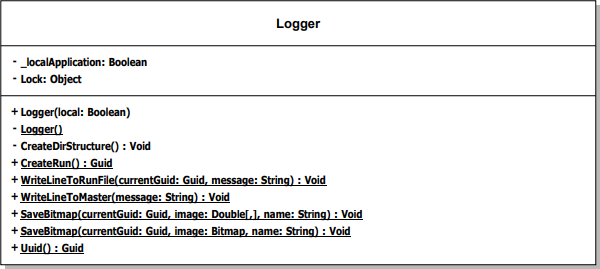
\includegraphics[width=12.5cm]{images/UML/Logger.png}}}
    \end{figure}\\

    \bk

    \paragraph{Logger Exception \textit{(Exception)}} \mbox{} \\

    \begin{figure}[H]
        \centering
        \subfloat[\centering Logger Exception Class Diagram]{{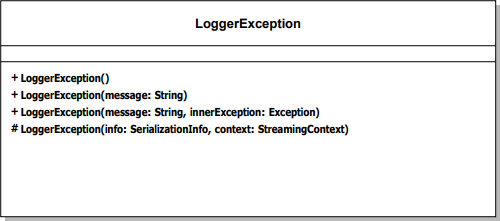
\includegraphics[width=12.5cm]{images/UML/LoggerException.png}}}
    \end{figure}\\

    \bk

    \paragraph{Map File \textit{(Class)}} \mbox{} \\

    \begin{figure}[H]
        \centering
        \subfloat[\centering Map File Class Diagram]{{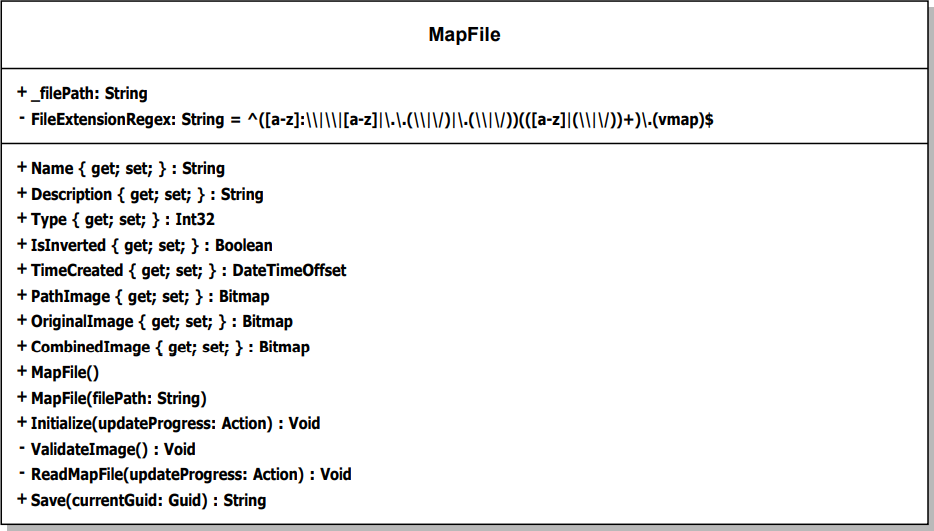
\includegraphics[width=12.5cm]{images/UML/MapFile.png}}}
    \end{figure}\\

    \bk


    \paragraph{Map File Exception \textit{(Exception)}} \mbox{} \\

    \begin{figure}[H]
        \centering
        \subfloat[\centering Map File Exception Class Diagram]{{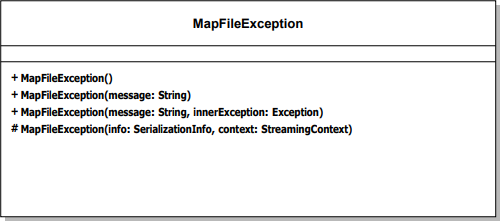
\includegraphics[width=12.5cm]{images/UML/MapFileException.png}}}
    \end{figure}\\

    \bk

    \paragraph{Matrix \textit{(Class)}} \mbox{} \\

    \begin{figure}[H]
        \centering
        \subfloat[\centering Matrix Class Diagram]{{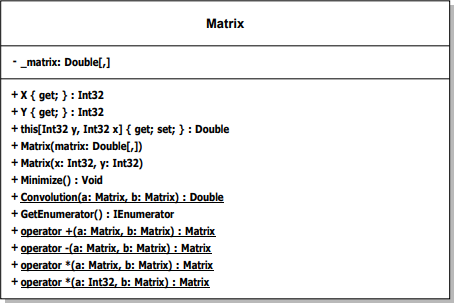
\includegraphics[width=12.5cm]{images/UML/Matrix.png}}}
    \end{figure}\\

    \bk

    \paragraph{Matrix Exception \textit{(Exception)}} \mbox{} \\

    \begin{figure}[H]
        \centering
        \subfloat[\centering Matrix Exception Class Diagram]{{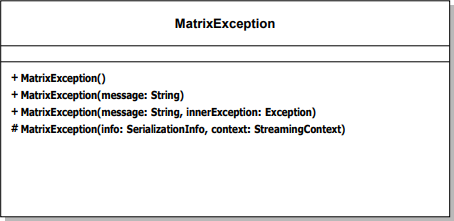
\includegraphics[width=12.5cm]{images/UML/MatrixException.png}}}
    \end{figure}\\

    \bk


    \paragraph{Max Priority Queue \textit{(Class)}} \mbox{} \\

    \begin{figure}[H]
        \centering
        \subfloat[\centering Max Priority Queue Class Diagram]{{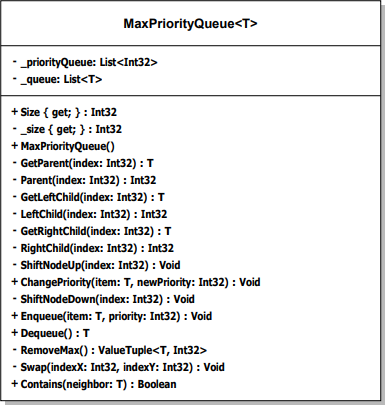
\includegraphics[width=12.5cm]{images/UML/MaxPriorityQueue.png}}}
    \end{figure}\\

    \bk

    \paragraph{Menu \textit{(Class)}} \mbox{} \\

    \begin{figure}[H]
        \centering
        \subfloat[\centering Menu Class Diagram]{{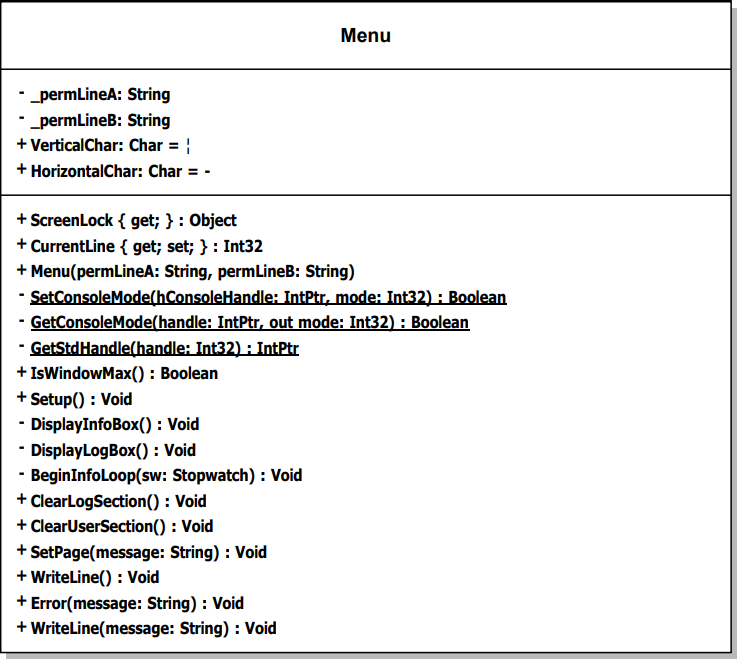
\includegraphics[width=12.5cm]{images/UML/Menu.png}}}
    \end{figure}\\

    \bk
    
    \paragraph{Min Priority Queue \textit{(Class)}} \mbox{} \\

    \begin{figure}[H]
        \centering
        \subfloat[\centering Min Priority Queue Class Diagram]{{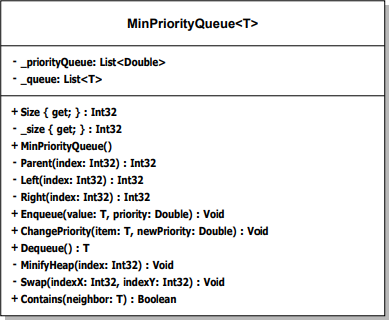
\includegraphics[width=12.5cm]{images/UML/MinPriorityQueue.png}}}
    \end{figure}\\

    \bk

    \paragraph{New Image \textit{(Class)}} \mbox{} \\

    \begin{figure}[H]
        \centering
        \subfloat[\centering New Image Class Diagram]{{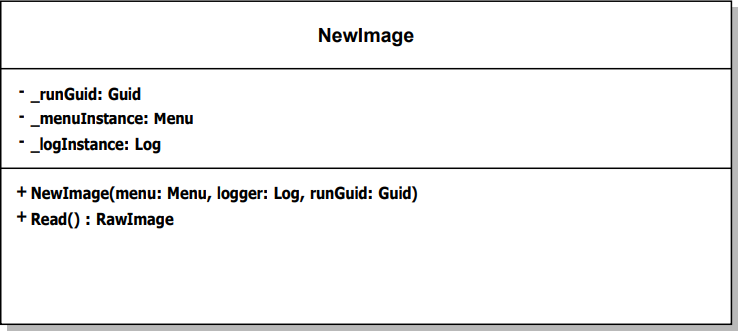
\includegraphics[width=12.5cm]{images/UML/NewImage.png}}}
    \end{figure}\\

    \bk

    \paragraph{Pathfinder \textit{(Class)}} \mbox{} \\

    \begin{figure}[H]
        \centering
        \subfloat[\centering Pathfinder Class Diagram]{{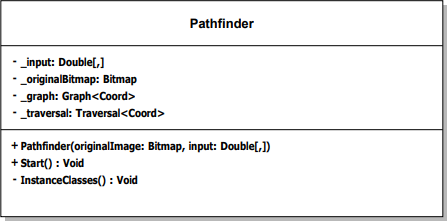
\includegraphics[width=12.5cm]{images/UML/Pathfinder.png}}}
    \end{figure}\\

    \bk

    \paragraph{Pathfind Image Form \textit{(Windows Form)}} \mbox{} \\

    \begin{figure}[H]
        \centering
        \subfloat[\centering Pathfind Image Form UML Diagram]{{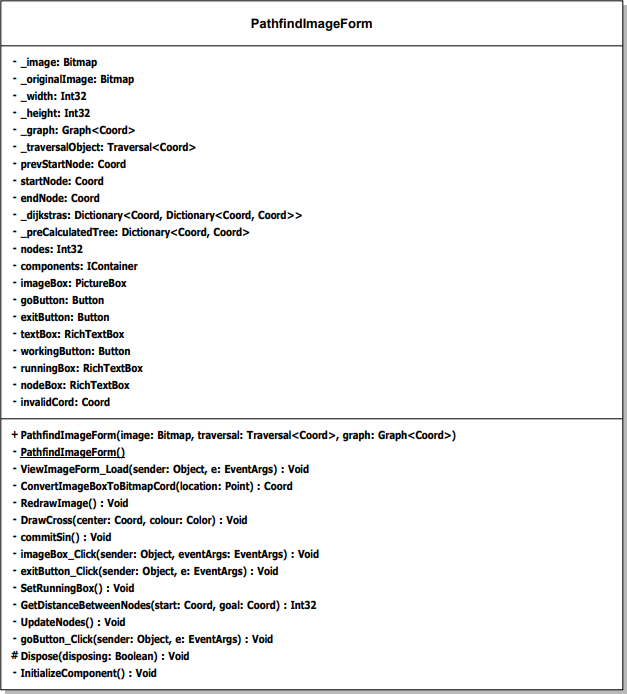
\includegraphics[width=12.5cm]{images/UML/PathfindImageForm.png}}}
    \end{figure}\\

    \bk

    \paragraph{Post \textit{(Class)}} \mbox{} \\

    \begin{figure}[H]
        \centering
        \subfloat[\centering Post Class Diagram]{{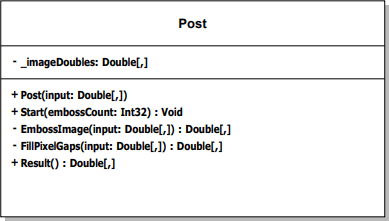
\includegraphics[width=12.5cm]{images/UML/Post.png}}}
    \end{figure}\\

    \bk

    \paragraph{Pre \textit{(Class)}} \mbox{} \\

    \begin{figure}[H]
        \centering
        \subfloat[\centering Pre Class Diagram]{{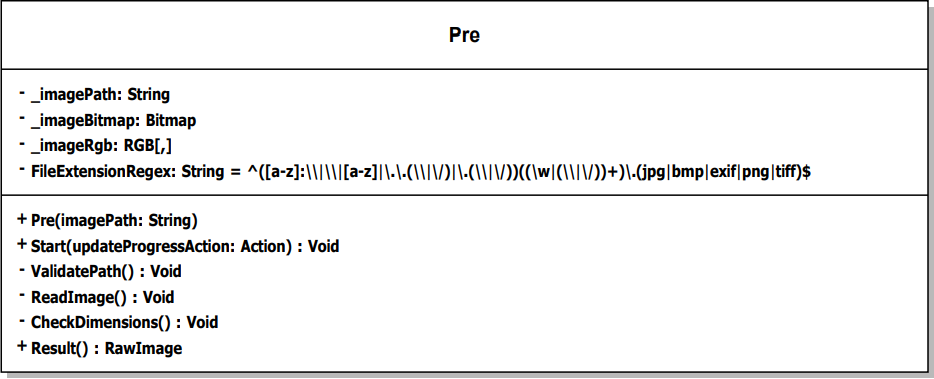
\includegraphics[width=12.5cm]{images/UML/Pre.png}}}
    \end{figure}\\

    \bk

    \paragraph{Preprocessing Exception \textit{(Exception)}} \mbox{} \\

    \begin{figure}[H]
        \centering
        \subfloat[\centering Preprocessing Exception Class Diagram]{{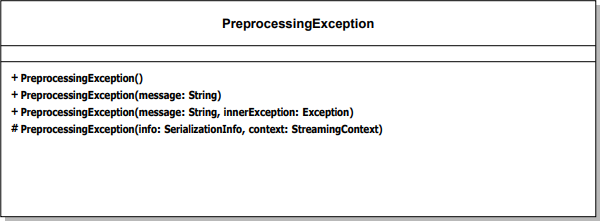
\includegraphics[width=12.5cm]{images/UML/PreprocessingException.png}}}
    \end{figure}\\

    \bk

    \paragraph{Program \textit{(Class)}} \mbox{} \\

    \begin{figure}[H]
        \centering
        \subfloat[\centering Program Class Diagram]{{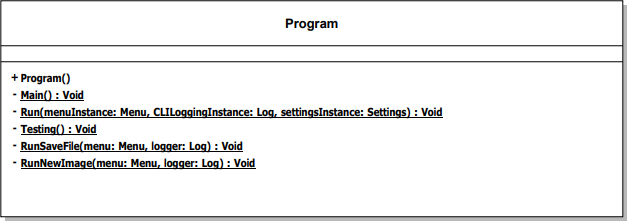
\includegraphics[width=12.5cm]{images/UML/Program.png}}}
    \end{figure}\\

    \bk

    \paragraph{Progress Bar \textit{(Class)}} \mbox{} \\

    \begin{figure}[H]
        \centering
        \subfloat[\centering Progress Bar Class Diagram]{{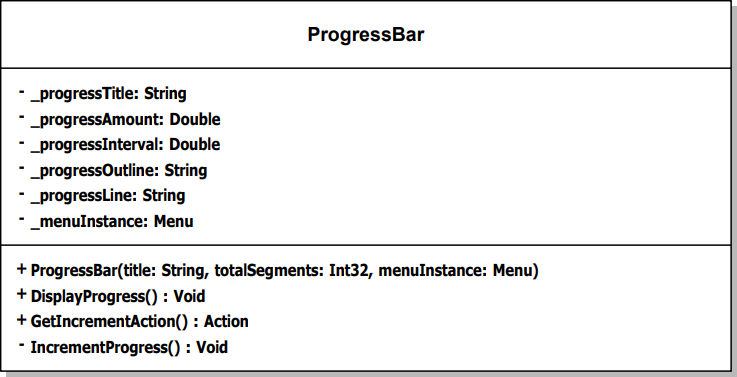
\includegraphics[width=12.5cm]{images/UML/ProgressBar.png}}}
    \end{figure}\\

    \bk

    \paragraph{Queue \textit{(Class)}} \mbox{} \\

    \begin{figure}[H]
        \centering
        \subfloat[\centering Queue Class Diagram]{{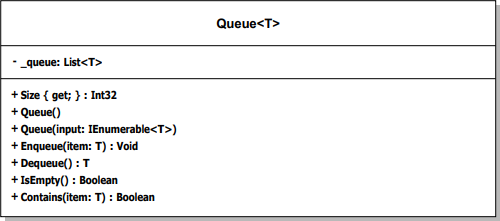
\includegraphics[width=12.5cm]{images/UML/Queue.png}}}
    \end{figure}\\

    \bk

    \paragraph{Raw Image \textit{(Structure)}} \mbox{} \\

    \begin{figure}[H]
        \centering
        \subfloat[\centering Raw Image Class Diagram]{{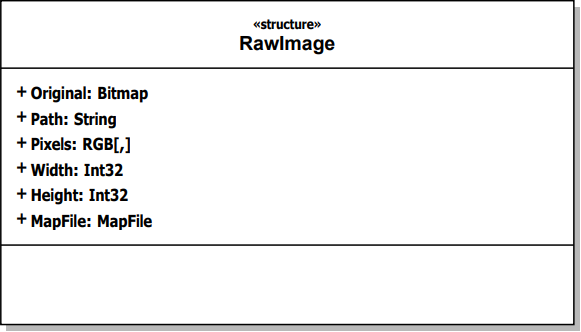
\includegraphics[width=12.5cm]{images/UML/RawImage.png}}}
    \end{figure}\\

    \bk

    \paragraph{RGB \textit{(Structure)}} \mbox{} \\

    \begin{figure}[H]
        \centering
        \subfloat[\centering RGB Class Diagram]{{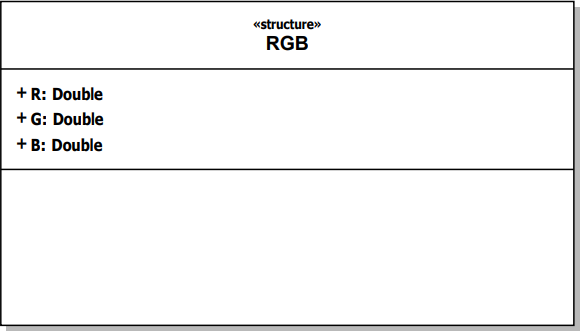
\includegraphics[width=12.5cm]{images/UML/RGB.png}}}
    \end{figure}\\

    \bk

    \paragraph{Road Detection \textit{(Class)}} \mbox{} \\

    \begin{figure}[H]
        \centering
        \subfloat[\centering Road Detection Class Diagram]{{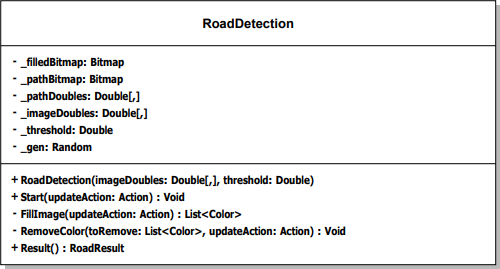
\includegraphics[width=12.5cm]{images/UML/RoadDetection.png}}}
    \end{figure}\\

    \bk

    \paragraph{Road Result \textit{(Structure)}} \mbox{} \\

    \begin{figure}[H]
        \centering
        \subfloat[\centering Road Result Class Diagram]{{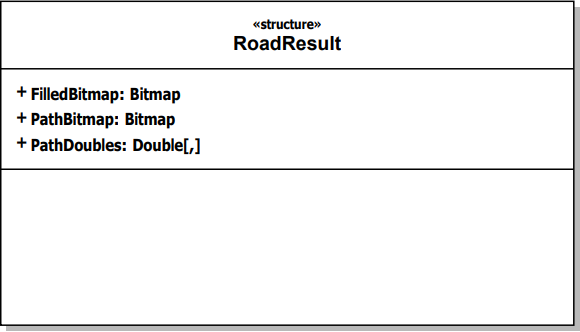
\includegraphics[width=12.5cm]{images/UML/RoadResult.png}}}
    \end{figure}\\

    \bk

    \paragraph{Road Sequence \textit{(Class)}} \mbox{} \\

    \begin{figure}[H]
        \centering
        \subfloat[\centering Road Sequence Class Diagram]{{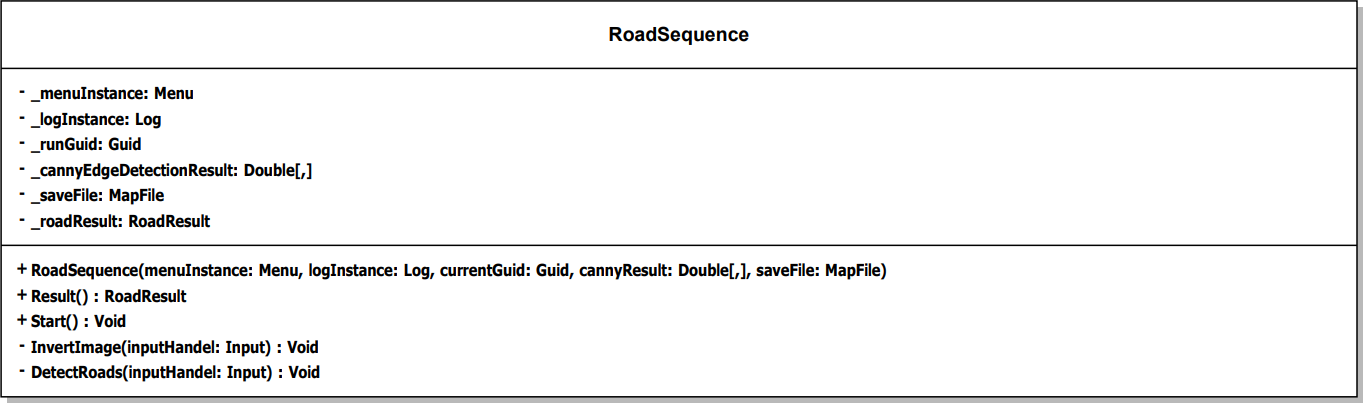
\includegraphics[width=12.5cm]{images/UML/RoadSequence.png}}}
    \end{figure}\\

    \bk

    
    \paragraph{Save File \textit{(Class)}} \mbox{} \\

    \begin{figure}[H]
        \centering
        \subfloat[\centering Save File Class Diagram]{{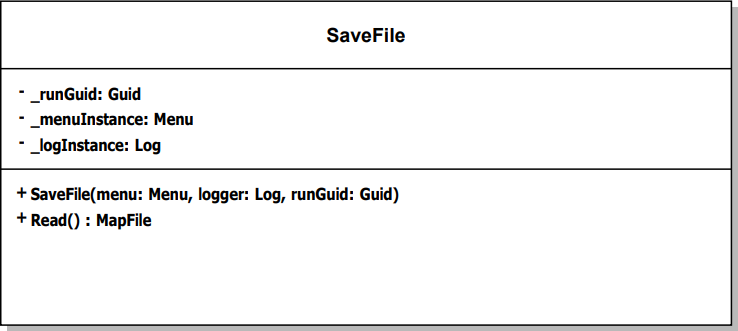
\includegraphics[width=12.5cm]{images/UML/SaveFile.png}}}
    \end{figure}\\

    \bk

    
    \paragraph{Settings \textit{(Class)}} \mbox{} \\

    \begin{figure}[H]
        \centering
        \subfloat[\centering Settings Class Diagram]{{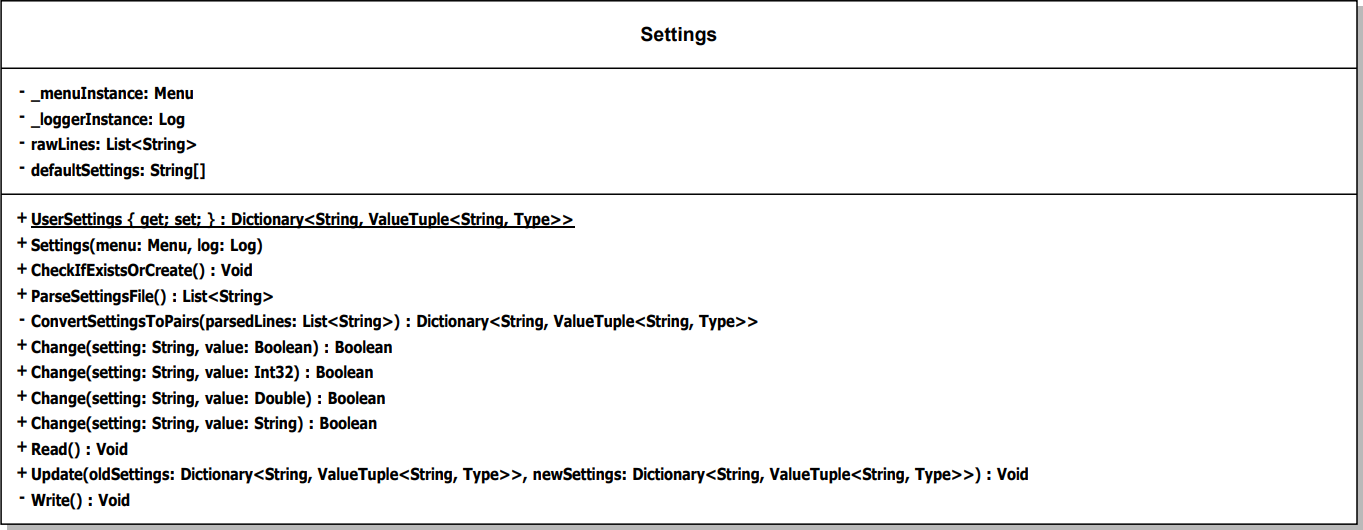
\includegraphics[width=12.5cm]{images/UML/Settings.png}}}
    \end{figure}\\

    \bk

    \paragraph{Settings Control \textit{(Class)}} \mbox{} \\

    \begin{figure}[H]
        \centering
        \subfloat[\centering Settings Control Class Diagram]{{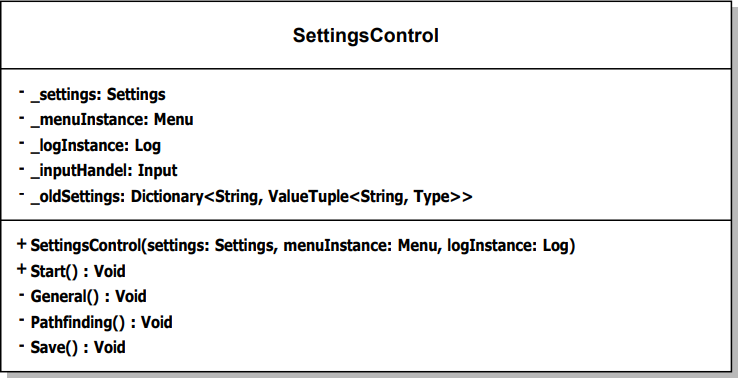
\includegraphics[width=12.5cm]{images/UML/SettingsControl.png}}}
    \end{figure}\\

    \bk

    \paragraph{Settings Exception \textit{(Exception)}} \mbox{} \\

    \begin{figure}[H]
        \centering
        \subfloat[\centering Settings Exception Class Diagram]{{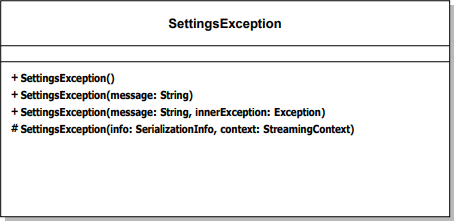
\includegraphics[width=12.5cm]{images/UML/SettingsException.png}}}
    \end{figure}\\

    \bk

    \paragraph{Stack \textit{(Class)}} \mbox{} \\

    \begin{figure}[H]
        \centering
        \subfloat[\centering Stack Class Diagram]{{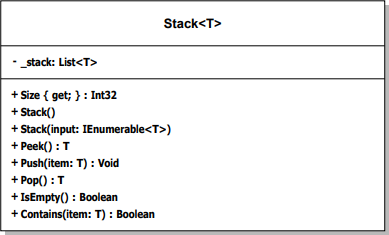
\includegraphics[width=12.5cm]{images/UML/Stack.png}}}
    \end{figure}\\

    \bk

    \paragraph{Structures \textit{(Class)}} \mbox{} \\

    \begin{figure}[H]
        \centering
        \subfloat[\centering Structures Class Diagram]{{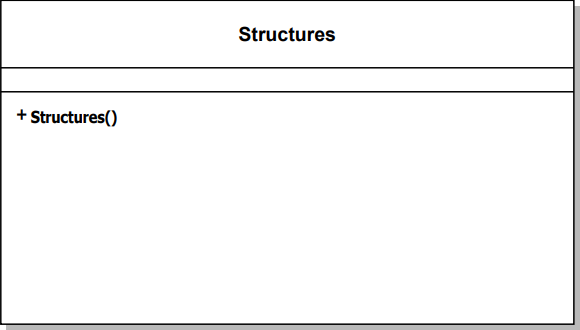
\includegraphics[width=12.5cm]{images/UML/Structures.png}}}
    \end{figure}\\

    \bk

    \paragraph{Sync Edge Detection \textit{(Class)}} \mbox{} \\

    \begin{figure}[H]
        \centering
        \subfloat[\centering Sync Edge Detection Class Diagram]{{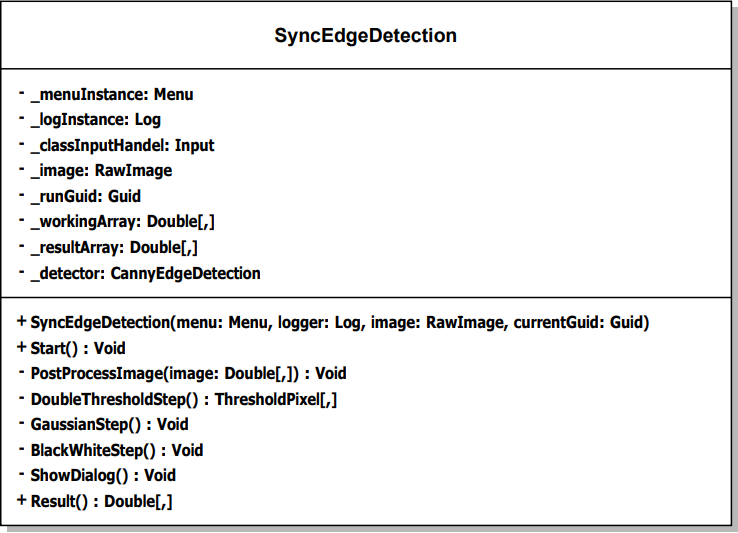
\includegraphics[width=12.5cm]{images/UML/SyncEdgeDetection.png}}}
    \end{figure}\\

    \bk


    \paragraph{Text Wall \textit{(Class)}} \mbox{} \\

    \begin{figure}[H]
        \centering
        \subfloat[\centering Text Wall Class Diagram]{{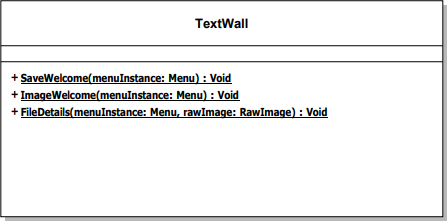
\includegraphics[width=12.5cm]{images/UML/TextWall.png}}}
    \end{figure}\\

    \bk

    \paragraph{Threshold Pixel \textit{(Structure)}} \mbox{} \\

    \begin{figure}[H]
        \centering
        \subfloat[\centering Threshold Pixel Class Diagram]{{\includegraphics[width=12.5cm]{images/UML/ThresholdPixel.png}}}
    \end{figure}\\

    \bk

    \paragraph{Traversal \textit{(Class)}} \mbox{} \\

    \begin{figure}[H]
        \centering
        \subfloat[\centering Traversal Class Diagram]{{\includegraphics[width=12.5cm]{images/UML/Traversal.png}}}
    \end{figure}\\

    \bk

    \paragraph{Utility \textit{(Class)}} \mbox{} \\

    \begin{figure}[H]
        \centering
        \subfloat[\centering Utility Class Diagram]{{\includegraphics[width=12.5cm]{images/UML/Utility.png}}}
    \end{figure}\\

    \bk

    \paragraph{View Image Form \textit{(Windows Form)}} \mbox{} \\

    \begin{figure}[H]
        \centering
        \subfloat[\centering View Image Form UML Diagram]{{\includegraphics[width=12.5cm]{images/UML/ViewImageForm.png}}}
    \end{figure}\\

    \bk

    








\end{flushleft}